\documentclass[tikz]{standalone}
\begin{document}
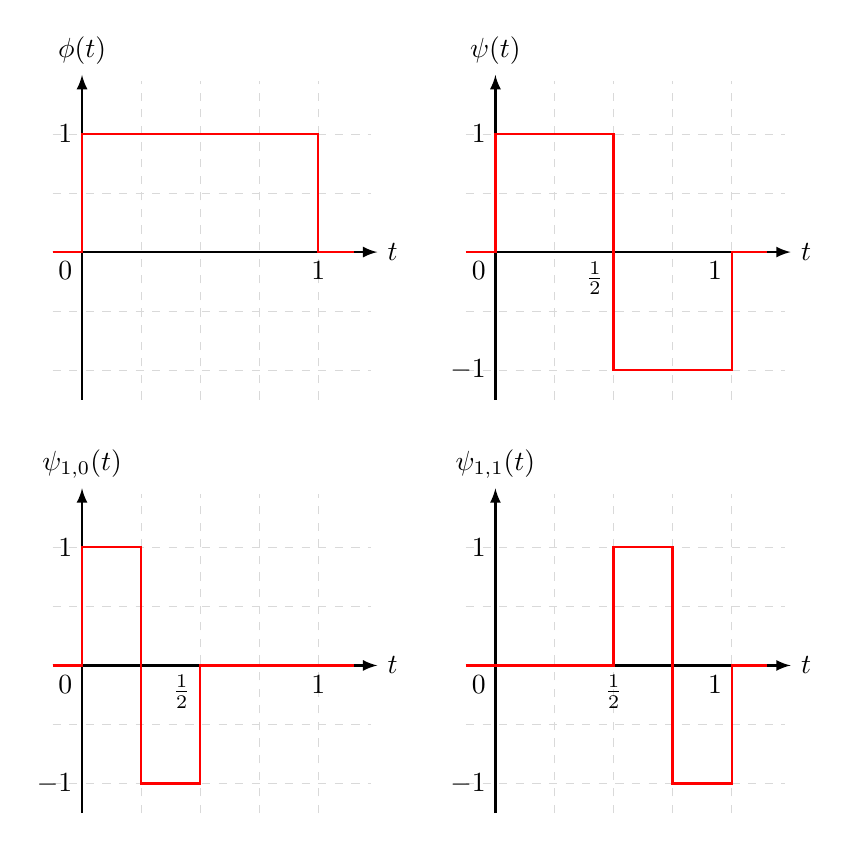
\begin{tikzpicture}[scale=0.75]
    \begin{scope}
    \draw[help lines, color=gray!30, dashed] (-.5,-2.5) grid (4.9,2.9);
    \draw[-latex,thick] (-.5,0)--(5,0) node[right]{$t$};
    \draw[-latex,thick] (0,-2.5)--(0,3) node[above]{$\phi(t)$};
    \draw[color=red,thick]
        (-.5,0) -- (0,0)
                -- (0,2)
                -- (4,2)
                -- (4,0)
                -- (4.6,0);
    \draw
        (0,0) node [anchor=north east] {$0$}
        (0,2) node [left] {$1$}
        (4,0) node [below] {$1$};
  \end{scope}
  \begin{scope}[shift={(7,0)}]
    \draw[help lines, color=gray!30, dashed] (-.5,-2.5) grid (4.9,2.9);
    \draw[-latex,thick] (-.5,0)--(5,0) node[right]{$t$};
    \draw[-latex,thick] (0,-2.5)--(0,3) node[above]{$\psi(t)$};
    \draw[color=red,thick]
        (-.5,0) -- (0,0)
                -- (0,2)
                -- (2,2)
                -- (2,-2)
                -- (4,-2)
                -- (4,0)
                -- (4.6,0);
    \draw
        (0,0) node [anchor=north east] {$0$}
        (0,2) node [left] {$1$}
        (0,-2) node [left] {$-1$}
        (2,0) node [anchor=north east] {$\frac{1}{2}$}
        (4,0) node [anchor=north east] {$1$};
  \end{scope}
  \begin{scope}[shift={(0,-7)}]
    \draw[help lines, color=gray!30, dashed] (-.5,-2.5) grid (4.9,2.9);
    \draw[-latex,thick] (-.5,0)--(5,0) node[right]{$t$};
    \draw[-latex,thick] (0,-2.5)--(0,3) node[above]{$\psi_{1,0}(t)$};
    \draw[color=red,thick]
        (-.5,0) -- (0,0)
                -- (0,2)
                -- (1,2)
                -- (1,-2)
                -- (2,-2)
                -- (2,0)
                -- (4.6,0);
    \draw
        (0,0) node [anchor=north east] {$0$}
        (0,2) node [left] {$1$}
        (0,-2) node [left] {$-1$}
        (2,0) node [anchor=north east] {$\frac{1}{2}$}
        (4,0) node [below] {$1$};
  \end{scope}
  \begin{scope}[shift={(7,-7)}]
    \draw[help lines, color=gray!30, dashed] (-.5,-2.5) grid (4.9,2.9);
    \draw[-latex,thick] (-.5,0)--(5,0) node[right]{$t$};
    \draw[-latex,thick] (0,-2.5)--(0,3) node[above]{$\psi_{1,1}(t)$};
    \draw[color=red,thick]
        (-.5,0) -- (2,0)
                -- (2,2)
                -- (3,2)
                -- (3,-2)
                -- (4,-2)
                -- (4,0)
                -- (4.6,0);
    \draw
        (0,0) node [anchor=north east] {$0$}
        (0,2) node [left] {$1$}
        (0,-2) node [left] {$-1$}
        (2,0) node [below] {$\frac{1}{2}$}
        (4,0) node [anchor=north east] {$1$};
  \end{scope}
\end{tikzpicture}
\end{document}